\documentclass[12pt]{article}
\usepackage{graphicx}
\usepackage{hyperref}
\usepackage{amsmath, amssymb}

\begin{document}

\title{Tarea 1}
\author{Entrega: 16 de junio, 2025}
\date{}
\maketitle

\begin{enumerate}

% =====================================================
\item En un juego de apuestas, empezás con un cierto número de fichas. En cada ronda, se lanza una moneda con probabilidad 0.53 de que salga cara. Si sale cara, perdés una ficha; si sale cruz, ganás una. Si perdés todas tus fichas, pagás \$10; si llegás a 10 fichas, ganás \$10.

    \begin{enumerate}
    \item Modele este juego como un proceso markoviano.
    \item Si empezás con 5 fichas, ¿cuál es tu ganancia esperada?
    \item ¿Con cuántas fichas al mínimo debés empezar para que la probabilidad de ganar sea mayor que la de perder?
    \item Ahora suponga que hay que llegar a 100 fichas para ganar. ¿Cómo cambia la respuesta anterior?
    \end{enumerate}

% =====================================================
\item Supongamos que un estudiante puede estar al día o atrasado. La probabilidad de su estado depende de las dos semanas anteriores:

    \begin{itemize}
        \item si estuvo atrasado dos semanas seguidas, estará atrasado con probabilidad 0.8;
        \item si estuvo al día dos semanas seguidas, estará al día con probabilidad 0.9;
        \item si estuvo atrasado y luego al día, estará atrasado con probabilidad 0.5;
        \item si estuvo al día y luego atrasado, estará atrasado con probabilidad 0.7.
    \end{itemize}

    \begin{enumerate}
    \item Modele la situación como un proceso markoviano.
    \item Si el estudiante estuvo al día el último mes, ¿cuál es la probabilidad de que esté atrasado en dos semanas?
    \item En el largo plazo, ¿qué fracción del tiempo está atrasado?
    \end{enumerate}

% =====================================================
\item Consideramos noticias sobre el mercado de telefonía móvil en Colombia:

\begin{center}
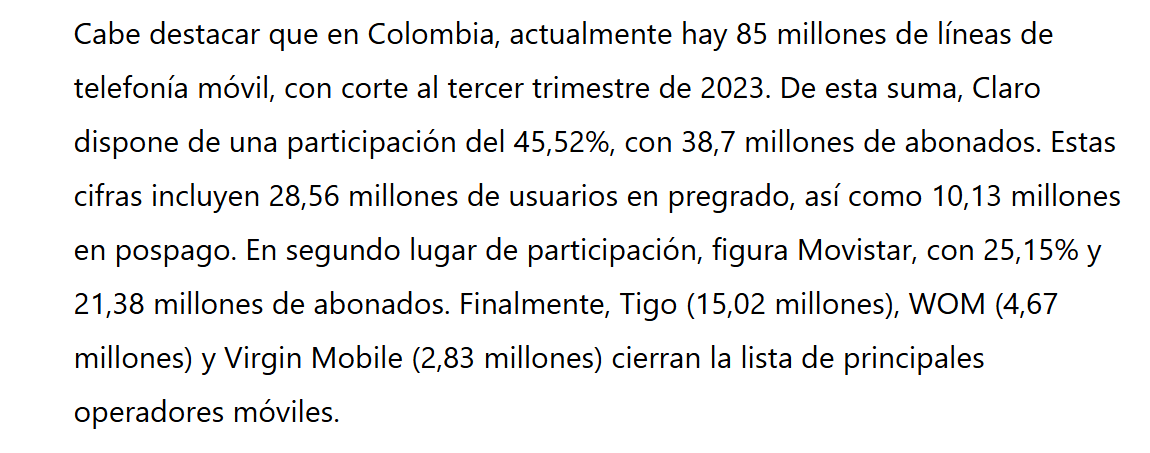
\includegraphics[width=0.9\textwidth]{../Images/MobilePhones/MobilePhoneMarket1.png}  

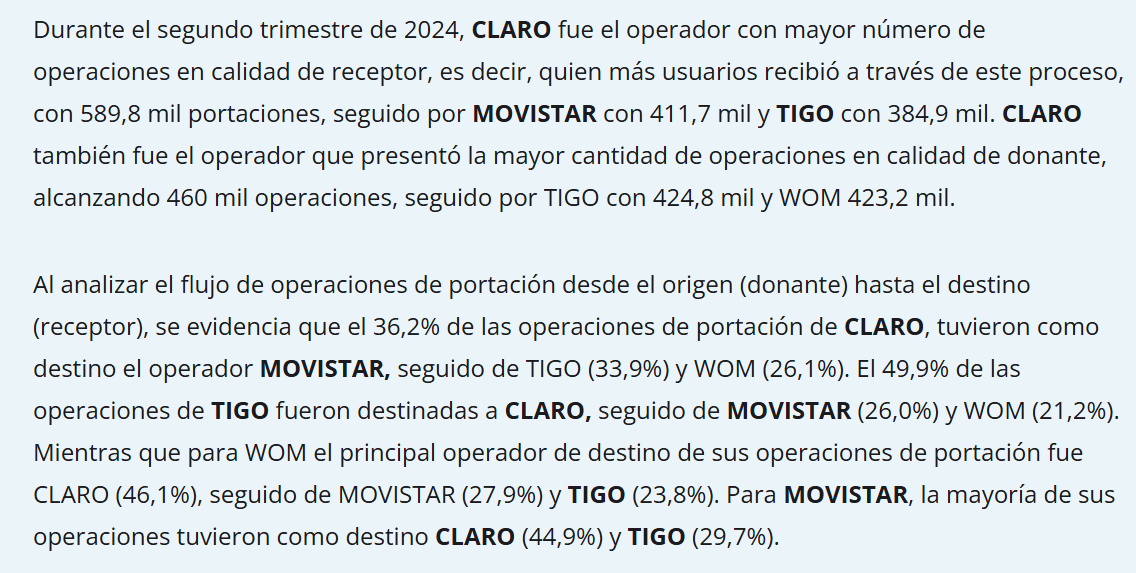
\includegraphics[width=0.9\textwidth]{../Images/MobilePhones/MobilePhoneMarket2.png} 
\end{center}

\begin{enumerate}
\item Complete la tabla con el número de usuarios al final del primer trimestre de 2024.

\item Estime los cambios de operador en el segundo trimestre y construya una matriz de transición. Explique cualquier supuesto.

\item En 2 años, ¿cuál es la participación de mercado esperada?

\item En equilibrio, ¿cuál es la participación de mercado?
\end{enumerate}

% =====================================================
\item \textbf{Modelo de inventario}

Consideramos el modelo visto en clase:

\[
X_{t+1} =
\begin{cases}
X_t - D_t & \text{si } X_t - D_t \ge n \\
N & \text{si } X_t - D_t < n
\end{cases}
\]

\begin{enumerate}

\item \textbf{Interpretación}
\begin{enumerate}
\item ¿Cómo interpreta el parámetro $n$? ¿Es razonable verlo como un “stock de seguridad”?
\item ¿Qué trade-off introduce este parámetro?
\end{enumerate}

\item \textbf{Transiciones}
\begin{enumerate}
\item Escriba la expresión de $P_{ij} = \mathbb{P}(X_{t+1} = j \mid X_t = i)$.
\item Explique cuándo ocurre una transición directa a $N$.
\end{enumerate}

\item \textbf{Exploración con código}

Utilizando el código de clase:

\begin{enumerate}
\item Compare la función valor para distintos valores de $n$.
\item Describa cómo cambia el comportamiento del sistema.
\end{enumerate}

\item \textbf{Discusión}
\begin{enumerate}
\item ¿Cómo elegiría $n$ en la práctica?
\item ¿Qué cambiaría si la demanda fuera más variable?
\end{enumerate}

\end{enumerate}

\end{enumerate}

\end{document}